\documentclass[12pt,letterpaper]{report}
\usepackage[margin=1in]{geometry}
\usepackage{graphicx}
\usepackage{amsmath}
\usepackage[font=small,labelfont=bf]{caption}
\usepackage[justification=centering]{caption}
\usepackage{tikz}
\usepackage{circuitikz}
\usepackage{siunitx}
\newlength \figwidth
\setlength \figwidth {0.75\linewidth}

\begin{document}

\title{E153 Laboratory Assignment \#3}
\author{Courtney Keeler and Stephen Pinto\\
Harvey Mudd College}
\date{October 21, 2013}
\maketitle

\section*{List of Materials}
\begin{itemize}
	\item Elenco LCM-1950 Multimeter
	\item 1N4001 diode
	\item standard value resistors
\end{itemize}

\section*{Purpose}
The purpose of this lab is to understand diodes and build circuits to measure the current through  a forward biased 1N4001 diode over ten orders of magnitude.

\section*{Procedure}

\begin{enumerate}
\item Construct the circuit shown in Figure \ref{fig:circuit_1}
\item Then we do this
\end{enumerate}

\begin{figure}
\centering
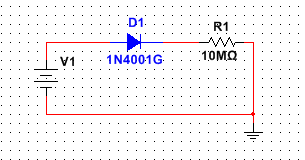
\includegraphics[width=\figwidth, keepaspectratio=true]{lab3/lab3_image_1.png}
\caption{Circuit to measure mid-range current values through the diode.}
\label{fig:circuit_1}
\end{figure}

\section*{Results}

\section*{Analysis}

\section*{Calculations}

\end{document}
